\documentclass[letterpaper, 12pt]{article}

\usepackage[spanish]{babel}
\usepackage[utf8]{inputenc}
\usepackage[T1]{fontenc}
\usepackage{graphicx}
\usepackage[hidelinks]{hyperref}

\pagestyle{headings}

\newcommand{\portada}[1][documentTitle]{
    \begin{titlepage}
	    \centering
    	
\includegraphics[width=0.30\textwidth]{src/img/escom}\par\vspace{1cm}
    	{\LARGE Instituto Politécnico Nacional \par}
	    {\Large Escuela Superior de Cómputo\par}
	    \vspace{1.5cm}
	    {\huge\bfseries #1 \par}
	    \vspace{2cm}
	    {\Large\itshape Valentin Ramos Emmanuel Guadalupe\par}
	    \vfill
	    Grupo: 1CM16\par
	    \vfill
	    {\large\today\par}
    \end{titlepage}
    \newpage
}

\begin{document}
    %Titulo del documento. (Portada)
    \portada[Tarea 02]
    %Contenido del documento.
    {\centering\section*{\LARGE El lenguaje C}\vspace{1cm}}
        \subsection*{Historia}
        El lenguaje C fue creado a mediados de los años 70 a manos de Brian Kernighan y Dennis Ritchie.
        Su primera implementación se realizó sobre el ordenador DEC PDP-11 con sistema operativo
        Unix por Dennis. C es el resultado de un proceso de desarrollo que comenzó con un lenguaje antecesor
        llamado BCPL, el cual influyó en el desarrollo por parte de Khen Thompson de un lenguaje llamado B, el 
        cual es considerado un antecedente de C. Desde su creación, surgieron varias versiones del lenguaje, que 
        incluían unas u otras características, palabras reservadas, etc. Fue uno de los lenguajes mas aceptados por
        los programadores, porque hace una conjugación en lenguaje de alto nivel y lenguaje máquina.\\
        En 1978 Kernighan y Ritchie publican su descripción en el libro  ``The C Programming Languaje", versión que hoy
        en día ``K\&R C". Este libro se suele llamar entre los programadores ``La biblia de C", existen varias ediciones y 
        en las universidades suele ser el libro principal de la bibliografía.
        A mediados de los ochenta, ya había en el mercado numerosos compiladores C, y muchas aplicaciones habían sido reescritas
        a él para aprovehchar sus ventajas.\\
        
        Finalmente, en 1980 Bjame Stroustrup de los maboratorios Bell de Murray Hill, New Jersey, adicionó las características de 
        la programación orientada a objetos y lo denominó C con clases. Para 1983 dicha denominación cambió a la de c++. Con este
        nuevo enfoque surge la nueva metodología que aumenta las posibilidades de la programación bajo nuevos conceptos.
        Con la posibilidad de las microcomputadoras se crearon muchas implementaciones de C. Sin embargo,
        como no existía ningún estándar, aparecieron discrepancias. Para remediar la situación, el instituto de
        Estándares Americano (ANSI) estableció un comité a mediados de 1983 para crear un estándar quedefiniera al lenguaje C. 
        Este comité ANSI termino el proceso de formalización en 1990. 

        \newpage
        \subsection*{Características}
        Originalmente el Lenguaje C estuvo muy ligado al sistema operativo UNIX como se había mencionado antes que, en su mayor parte, está escrito en C. 
        Más adelante se comenzó a utilizar en otros sistemas operativos para programar editores, compiladores, etc. Aunque se le conoce como un lenguaje de programación de sistemas, 
        no se adapta mal al resto de aplicaciones. De hecho, hoy en día un alto porcentaje de software para ordenadores personales está escrito en Lenguaje C. Por ejemplo, el sistema operativo MS-DOS.\\
        Algunas de las características más importantes que definen el lenguaje y que han permitido que sea tan popular, como lenguaje de programación son: 
        \begin{itemize}
            \item Tiene un conjunto completo de instrucciones de control.
            \item Permite la agrupación de instrucciones.
            \item Incluye el concepto de puntero
            \item Los argumentos de las funciones pueden transferirse por su valor.
            \item Posiblidad de ser compilado en variedad de ordenadores con pocos cambios (Portabilidad).
            \item Manejo de actividades de bajo-nivel.
        \end{itemize}

        \subsection*{Algunos modificadores de tipos de datos}
        En C, toda variable y/o constante, antes de poder ser usada, debe ser declarada especificanco del tipo de dato que almacenará.
        Toda variable en C se declara de la forma:
        
        \begin{verbatim}
            <tipo_de_dato> <nombre_de_la_variable>;
        \end{verbatim}

        Por citar algunos ejemplos:

        \begin{verbatim}
            float miNumeroFlotante;
            int miEntero1, miEntero2;
            char miCaracter, otroCaracter;
        \end{verbatim}

        Existen, además cuatro modificadores de tipo, los cuales se aplican sobre los tipos de datos anteriormente
        mencionados. Estos modificadores permiten cambiar el tamaño, etc., de los otros tipos.
        Estos modificadores, que sintacticamente anteceden a la declaración del tipo de dato, son:
            
        \begin{center}
            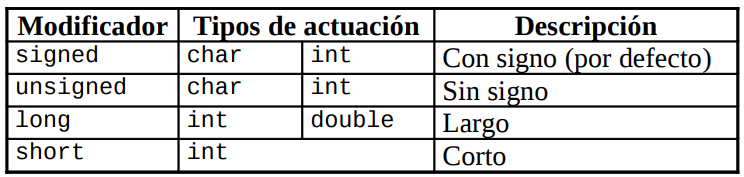
\includegraphics[width=0.9\textwidth]{src/img/table1.png}
        \end{center}

        Gracias a ello, podemos tener variables como:

        \begin{verbatim}
            unsigned char miChar;
            long double myDouble;
            short int myInt;
        \end{verbatim}

        Es posible, además, aplicar dos modificadores seguidos a un mismo tipo de
        datos, así, es posible definir una variable de tipo unsigned long int (entero largo sin
        signo). El rango de valores de que permite cada variable depende del sistema operativo
        sobre el cual se trabaje (MS-DOS, Windows95/98/NT/2000, UNIX/Linux).

        \begin{center}
            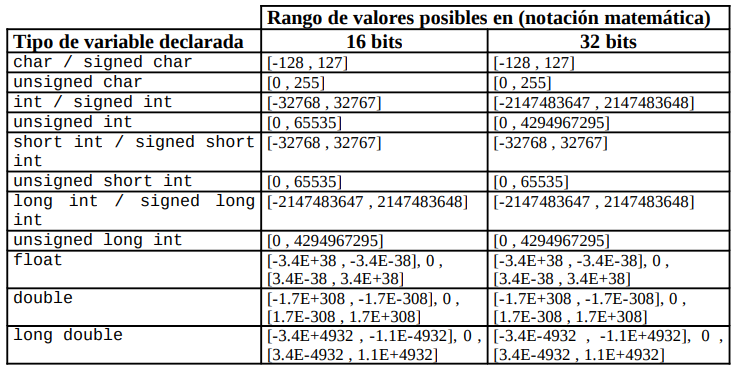
\includegraphics[width=0.9\textwidth]{src/img/table2.png}
        \end{center}

        Estos valores pueden diferir, así que para información mas precisa, se debe revisar la documentación
        del compilador utilizado.

        \newpage

        \begin{thebibliography}{0}
            \bibitem{Brian1991} Kernighan W. B. y Ritchie M. D. (1991). El lenguaje de programación C. Pearson Educación. \href{https://tinyurl.com/yd7z69n3}{(https://tinyurl.com/yd7z69n3)}
            \bibitem{Enrique} Enrique Vicente B. E. (s. f.) Lenguaje C. \href{https://tinyurl.com/y34mnogc}{(https://tinyurl.com/y34mnogc)}
        \end{thebibliography}


\end{document}